\documentclass[12pt]{article}
\usepackage[a4paper,bindingoffset=0.2in,left=2.5cm,right=2.5cm,top=1.5cm,bottom=1.5cm,footskip=.25in]{geometry}
\usepackage{graphicx}
\usepackage{caption}
\usepackage{subcaption}
\usepackage{placeins}
\usepackage{amsmath}
\usepackage{hyperref}

%================================
\title{Detection of IC, FO. Velocity and Position Estimate using ZUPT and Kalman Filter}
\author{Sandeep Kumar, Laura Rocchi, K. Gopinath, Poorna T. S.\\
CSA, Indian Institute of Science\\
Robert Bosch Center for Cyber Physical Systems, IISc
}


\begin{document}
\maketitle

\section*{Introduction}
This brief report contains the method used to detect IC (Initial Contact) and FO (Foot Off) using the data gathered from placing an IMU sensor on the foot. We also used this data, specifically the Accelerometer data from the foot to calculate the velocity and  position of the user \footnote{All the results shown hence forward are for walk number 20 (EXL IMU sensor labeling)}. A ZUPT (Zero Velocity Update ) algorithm along with a Kalman filter was used to remove the drift which creeps in because of the noise present in the accelerometer data.

\section*{Initial Contact and Foot Off}
Detecting IC and FO is one of the most important gait feature. Once we have an accurate estimate of IC and FO, we can use that information to detect other gait features, such as Step length, Gait Speed, Gait asymmetry etc. We are using the method mentioned in \cite{s140406229} for this purpose.

The primary purpose of the paper \cite{s140406229} is to build a wearable system for Gait training for people with Parkinson's disease. They placed IMU sensors on the foot of the patient and used the Gyroscope data along the mediolateral axis (The axis of rotation, in our case it was the X axis of the sensors).

\begin{figure}[!htb]
\centering
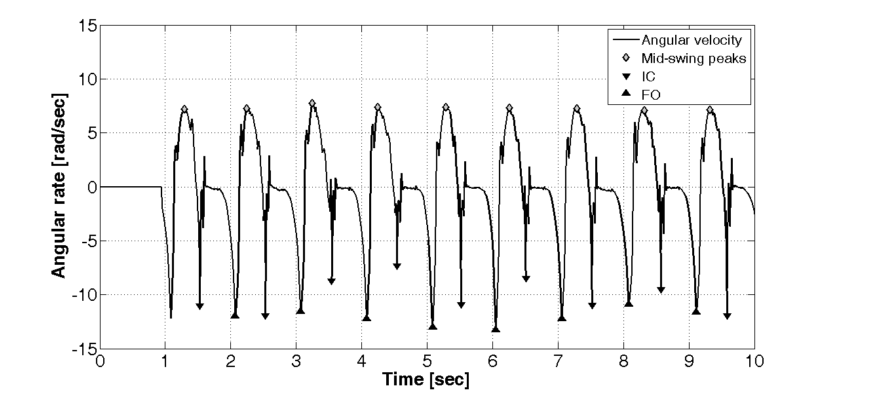
\includegraphics[scale=.4]{ictodetection.png}
\caption{Detection of IC and FO as per \cite{s140406229} \\
}
\label{icnadtodetection}
\end{figure}

\FloatBarrier 

\subsection*{Algorithm}

\begin{verbatim}
Using the Angular Velocity along the axis of rotation of foot.
1. Identify all positive peaks (anti clockwise direction, looking from
   right side), associated with mid-swing events.
2. Identify all the negative peaks
3. With each couple of mid swing peaks,
   a. First Negative Peak (clockwise direction) is the IC.
   b. Second Negative Peak is the FO.

\end{verbatim}

An on-line version of the current algorithm was presented in \cite{7173053}. In this paper they tune the parameter to detect the peaks, like 'Minimum Peak Height', 'Minimum Peak Distance' automatically from the data. They start with some default initial values (based on the filter and subject) then they update it after every fourth step.

\begin{verbatim}
SF <- sampling frequency
gyrT <- 1
timT <- SF/7
For Positive Peaks
    minPeakHeight = gyrT;
    minPeaksDistance = timT/2;
For Negative Peaks
    minPeakHeight = gyrT * 0.2;
    minPeakDistance = timT/5;
    
Every 4 steps
    gyrT <- median(positivePeaks)^(0.7)
    timT <- median(positivePeaks(i+1)-positivePeaks(i))/3
\end{verbatim}

We had to tweak the default values a little to suit our sensors
\begin{verbatim}
gyroT = 5;
freq=100;

For Positive Peaks
    minPeakHeight = gyroT;
    minPeakDistnace = ceil(freq/7);
For Negative Peaks
    minPeakHeight = ceil(gyroT*0.2);
    minPeakDistnace = ceil(freq/7);
\end{verbatim}

There were some extra conditions that were enforced, like a IC and FO can only occur between two same positive peaks.
\begin{figure}[!htb]
\centering
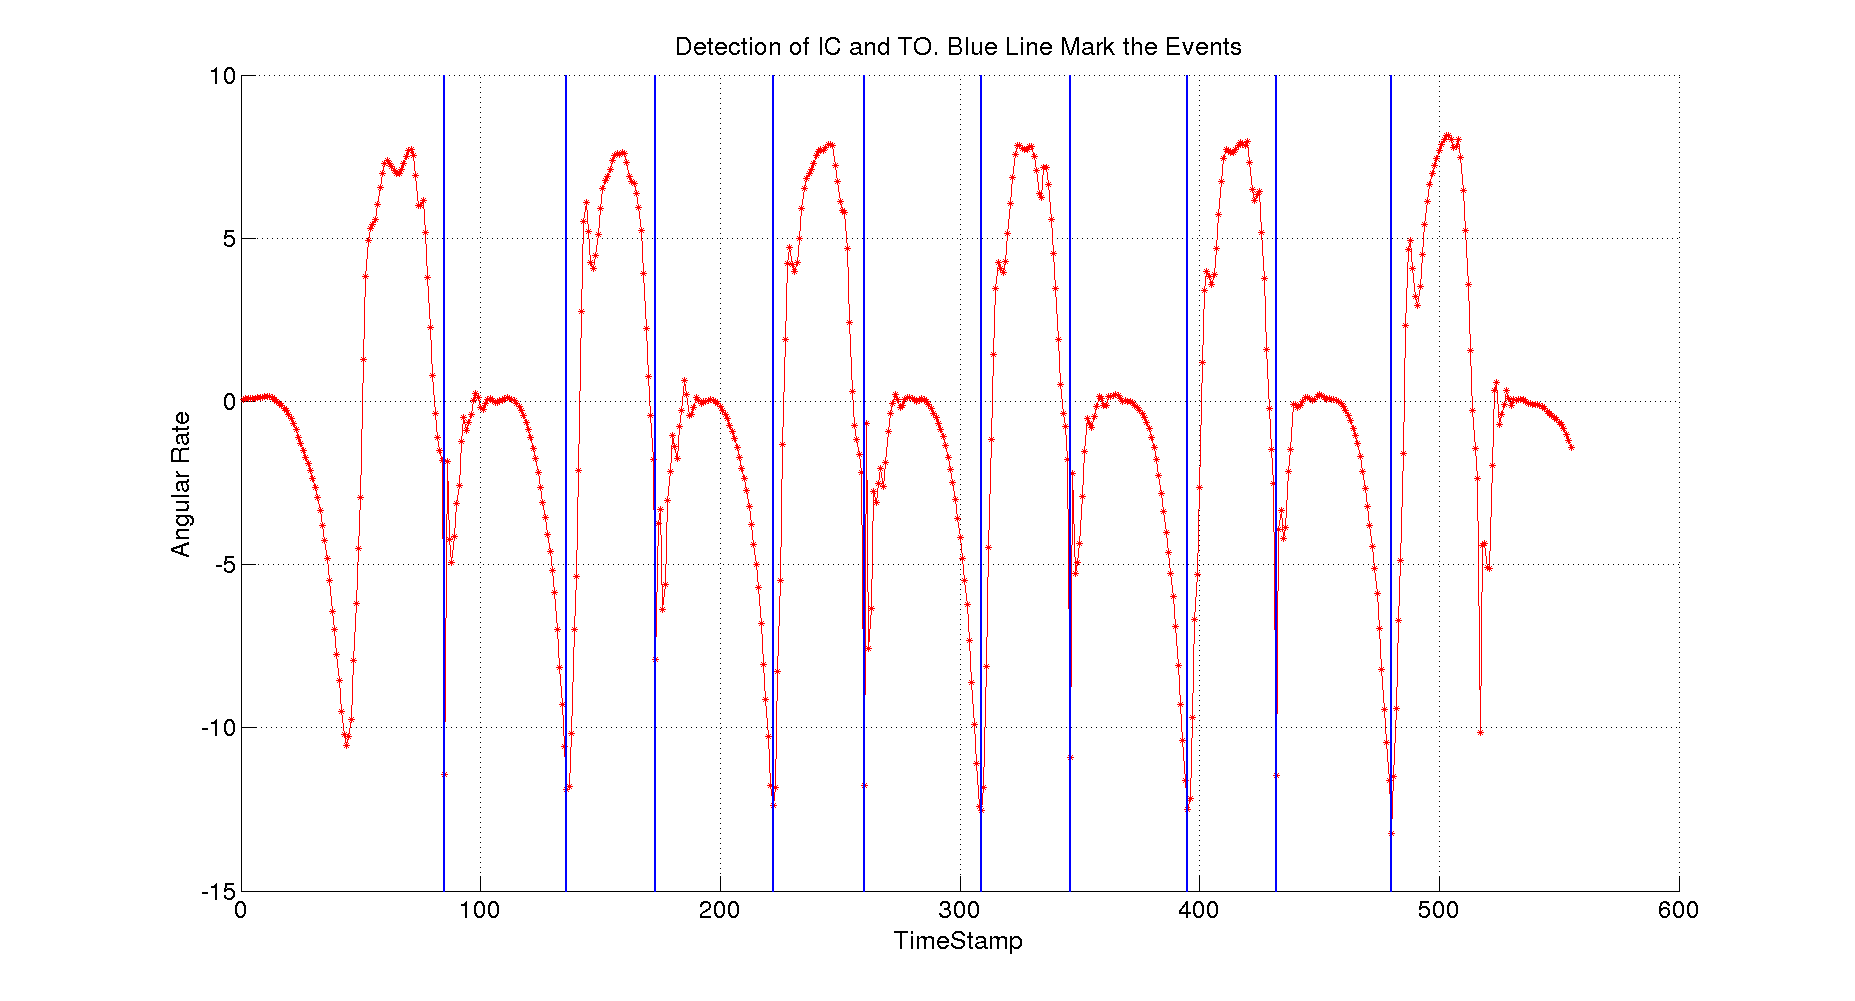
\includegraphics[scale=.3]{ourictodetection.png}
\caption{Detection of IC and FO on our data \\
}
\label{ouricnadtodetection}
\end{figure}
\FloatBarrier

\section*{Velocity and Position}

The acceleration data collected by the IMU sensors is shown in the figure \ref{acceleration}.
\begin{figure}[!htb]
\centering
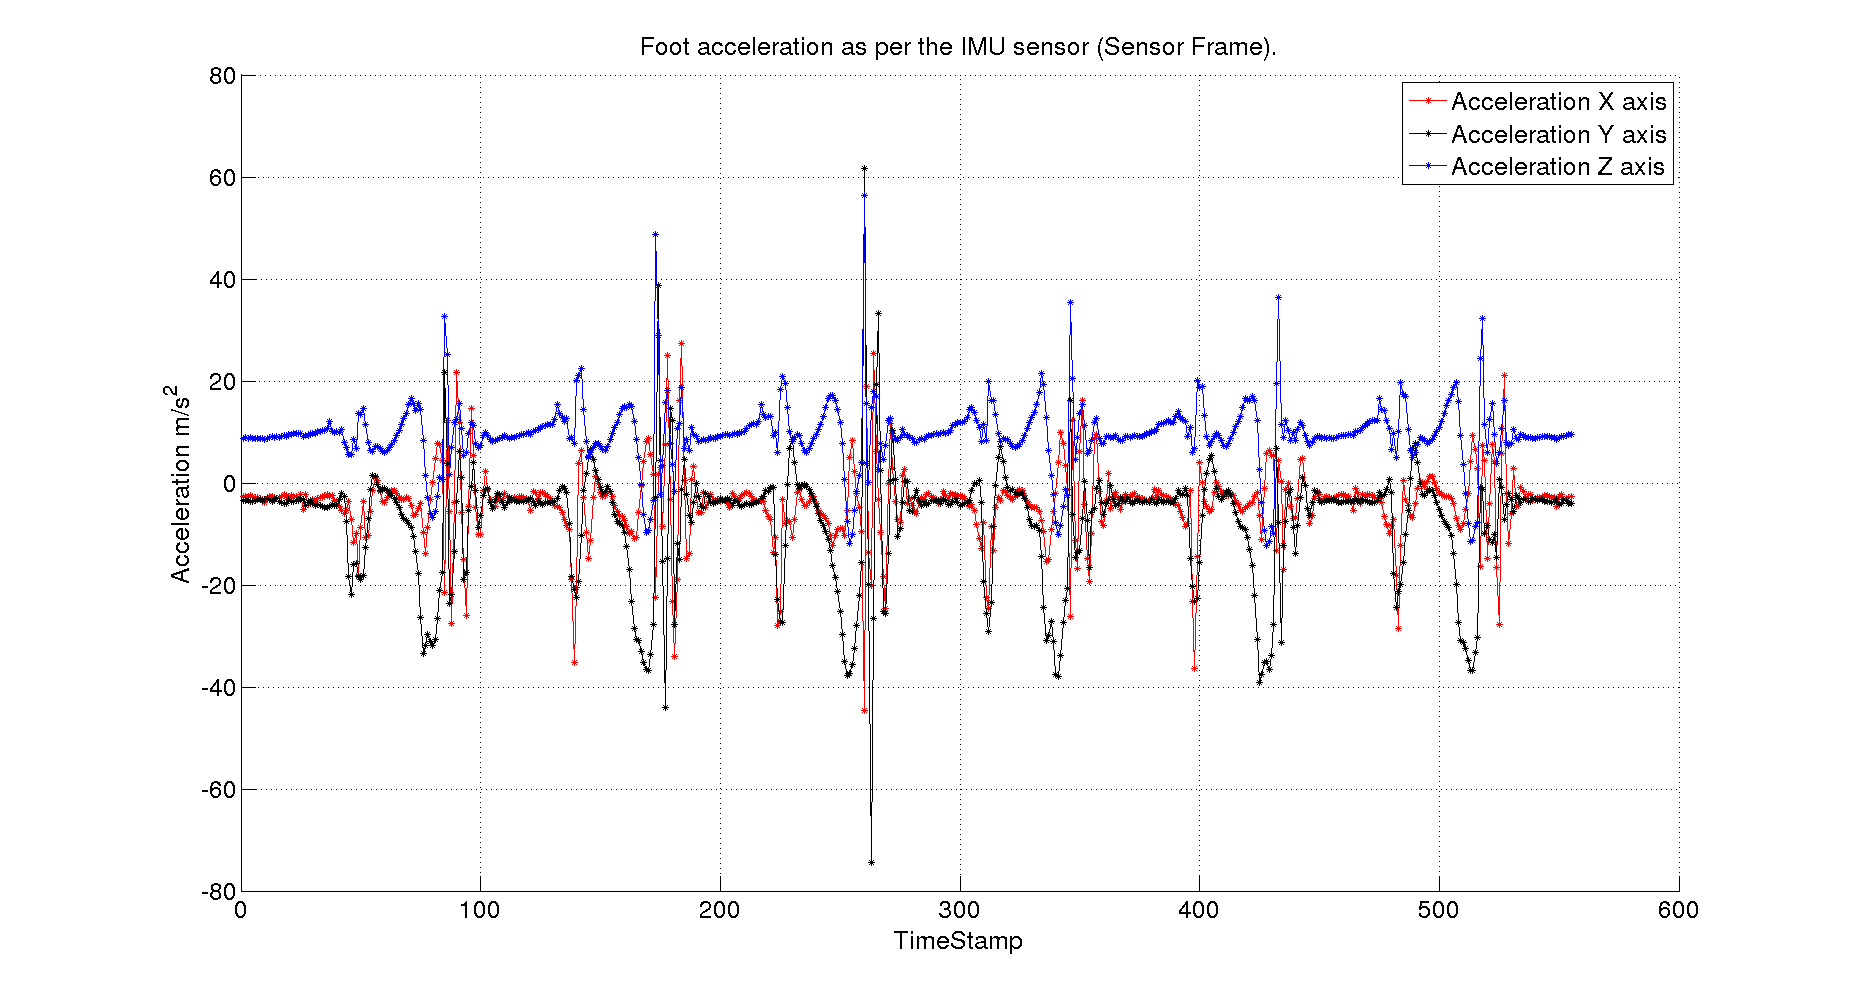
\includegraphics[scale=.3]{acceleration.png}
\caption{Acceleration}
\label{acceleration}
\end{figure}

To calculate the velocity from the acceleration data, we followed the steps mentioned in the tutorial \cite{6127851}. The main steps are:
\begin{itemize}
\item Transform accelerations from sensor frame to navigation frame by using the sensor orientation data.
\item Subtract the gravity
\item Integrate Acceleration to obtain velocities.
\end{itemize}

\begin{figure}[!htb]
\centering
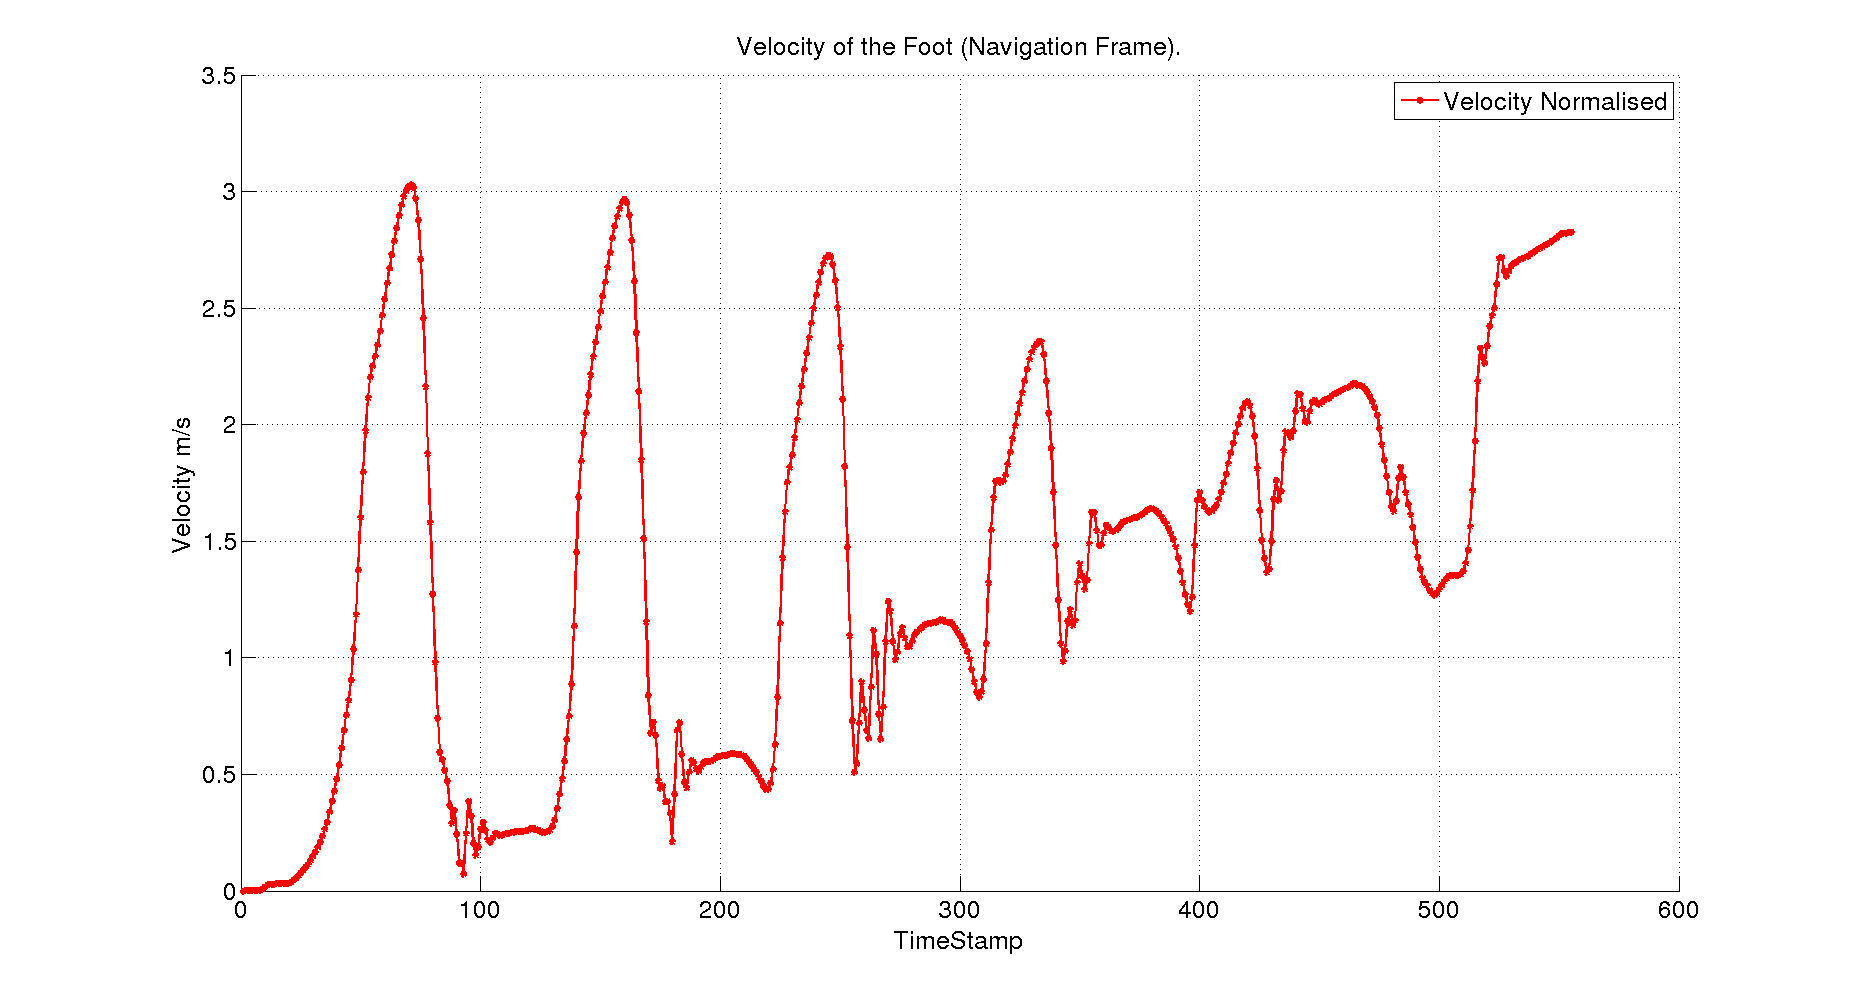
\includegraphics[scale=.3]{velocityDrift.png}
\caption{Velocity with Drift}
\label{velocityDrift}
\end{figure}

\FloatBarrier

We can see that there is drift present in the data because of the noise in the accelerometer data. One way to correct this drift, is to use the information the during the stance phase the velocity of the foot is zero.

\begin{figure}[!htb]
\centering
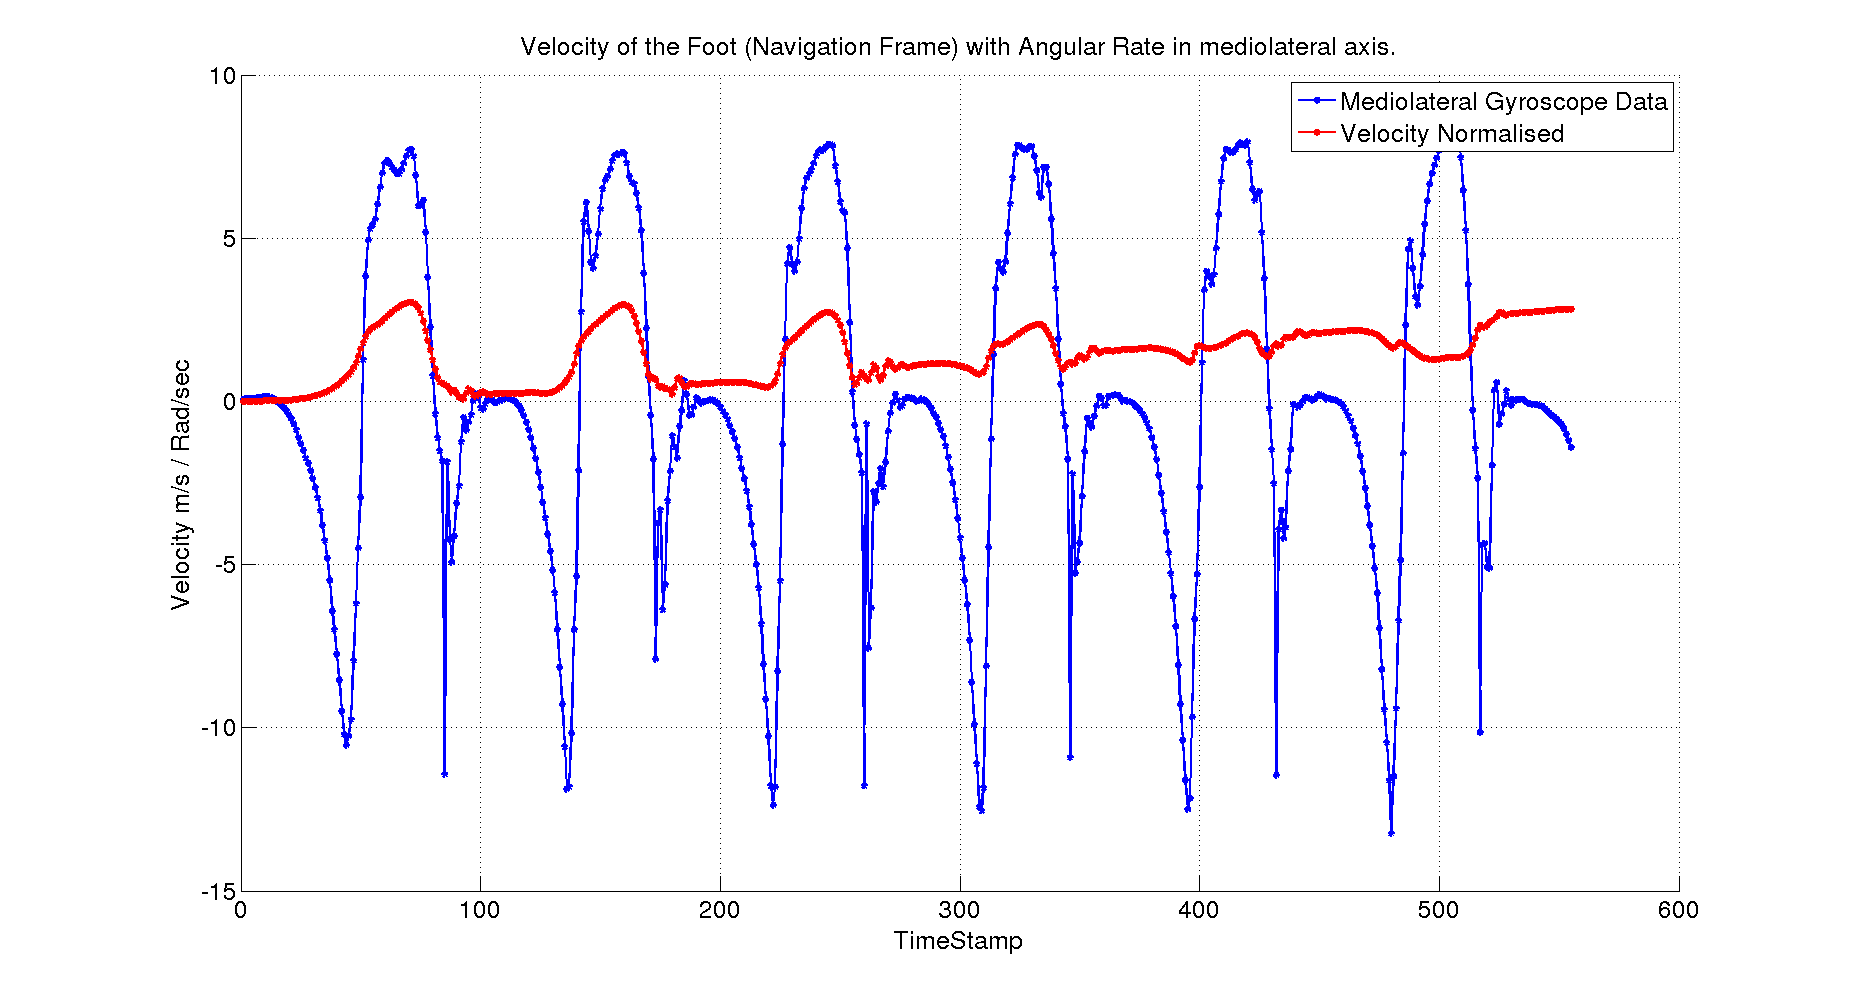
\includegraphics[scale=.3]{velocityDriftGyro.png}
\caption{Velocity with Drift and Gyroscope Data for Mediolateral Axis}
\label{velocityDriftGyro}
\end{figure}

\FloatBarrier

\subsubsection*{Zero Velocity Detection}
Now  during stance phase also, the foot is not completely at rest for all the time. \cite{5646936} gives some statistical techniques which can be used to define the period in which the foot is completely at rest.\\\\
$ y_n^a \in \mathbf{R}^3 $  and $ y_n^{\omega} \in \mathbf{R}^3 $ is the acceleration and angular velocity respectively. \\
The objective of the zero-velcoty detector is to determine whether, during a time epch consisting of $ W \in \mathbf{N} $ observations between the time instants \textit{n} and \textit{n+W-1}, the IMU is moving or stationary.\\\\
\begin{equation}
 z_n^a = \{y_k^a\}_{k=n}^{n+W-1} ;
 z_n^{\omega} = \{y_k^\omega\}_{k=n}^{n+W-1}
\end{equation}
\\\\
\underline{The Stance Hypothesis Optimal Detector (SHOE)}
\begin{equation}
T(z_n^a,z_n^{\omega})=\frac{1}{W} \sum_{k=n}^{n+w-1}\frac{1}{\sigma_a^2}||y_k^a-g\frac{\bar{y}_n^a}{||\bar{y}_n^a||}||^2 +\frac{1}{\sigma_{\omega}^2}|||y_k^{\omega}||^2
\end{equation}

\underline{The Acceleration Moving Variance Detector (MV)}
\begin{equation}
T(z_n^a,z_n^{\omega})=\frac{1}{\sigma_a^2W} \sum_{k=n}^{n+w-1}||y_k^a-\bar{y}_n^a||_2
\end{equation}

\underline{The Acceleration Magnitude Detector (MAG)}
\begin{equation}
T(z_n^a,z_n^{\omega})=\frac{1}{\sigma_a^2W} \sum_{k=n}^{n+w-1}(||y_k^a||-g)^2
\end{equation}

\underline{The Angular Rate Energy Detector (ARE)}
\begin{equation}
T(z_n^a,z_n^{\omega})=\frac{1}{\sigma_a^2W} \sum_{k=n}^{n+w-1}||y_k^\omega||^2
\end{equation}

IMU is stationary if
\begin{equation}
T(z_n^a,z_n^{\omega})< \gamma
\end{equation}
$ \gamma $ is the detection threshold.\\
Determining the value of W and $ \gamma $ is another problem.

\begin{figure}[!htb]
\centering
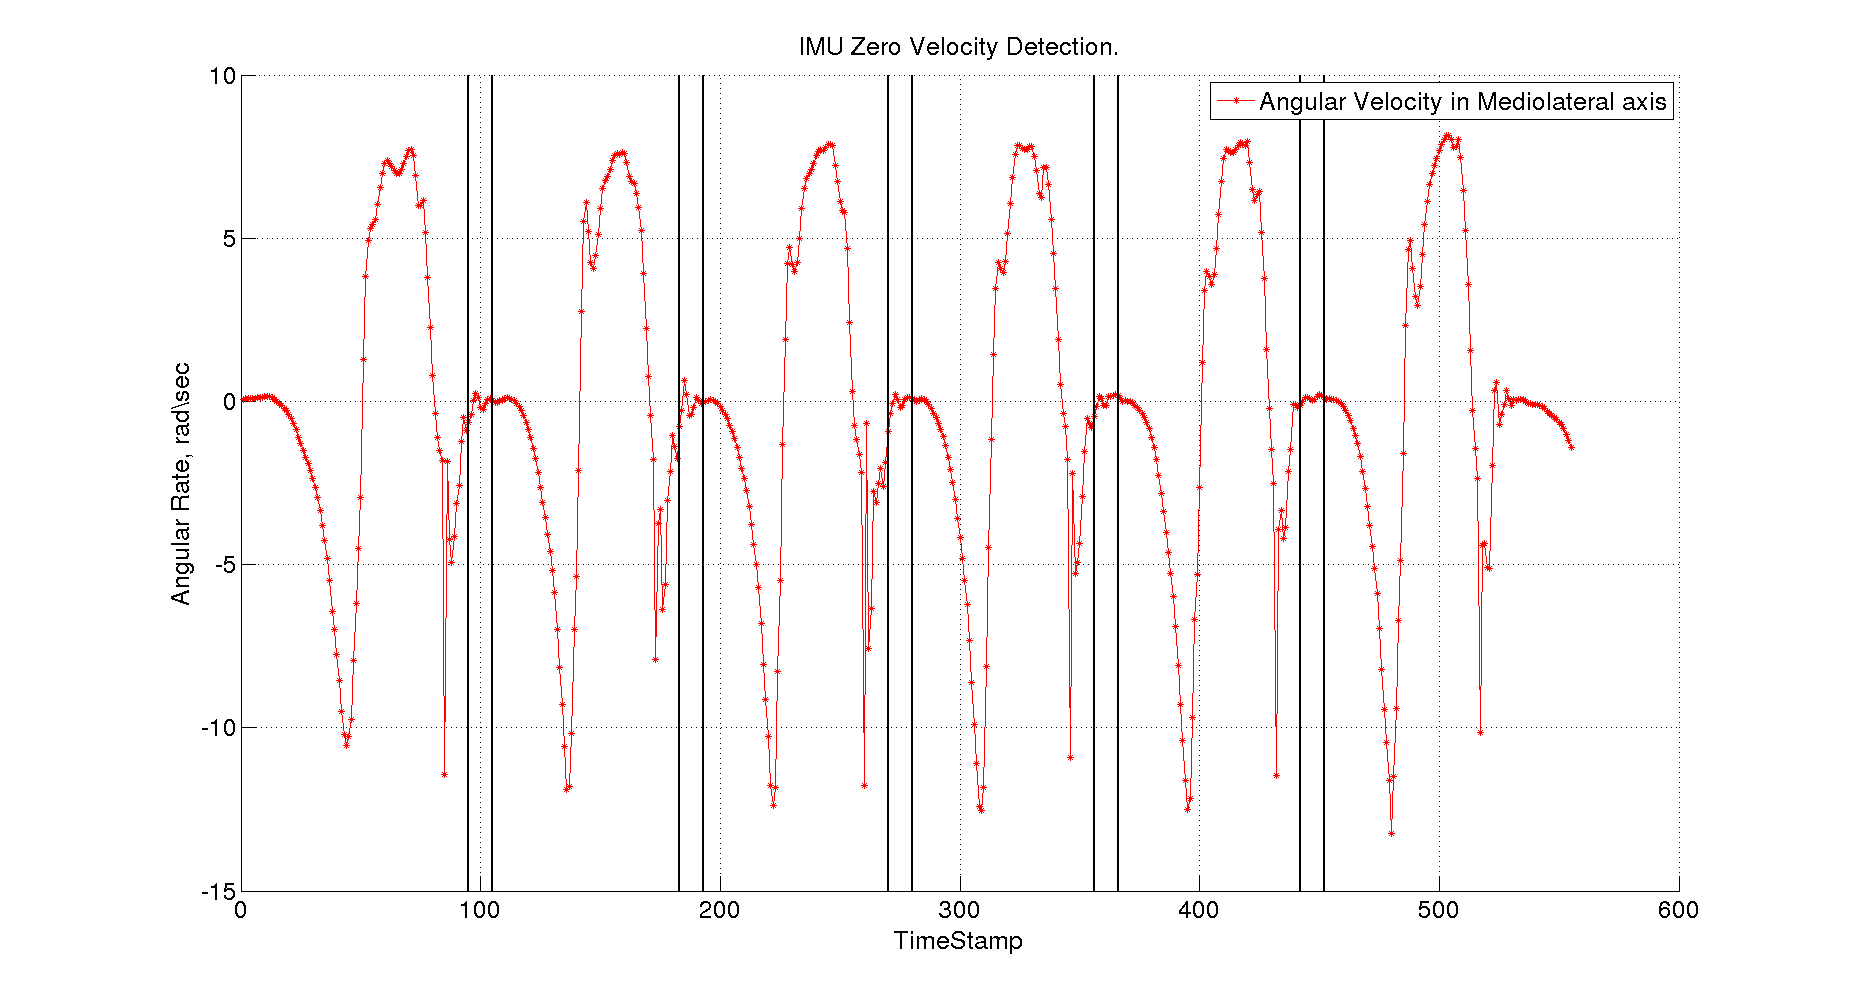
\includegraphics[scale=.3]{imuzerovelocity.png}
\caption{IMU Zero Velocity Detection. Using SHOE. W=10}
\label{imuzerovelocity}
\end{figure}

\FloatBarrier

Another method, which is much more simple, is just to use the Gyroscope values.
\begin{verbatim}
gyro_threshold = 0.7;
norm(gyro_s(:,n)) < gyro_threshold
\end{verbatim}

\begin{figure}[!htb]
\centering
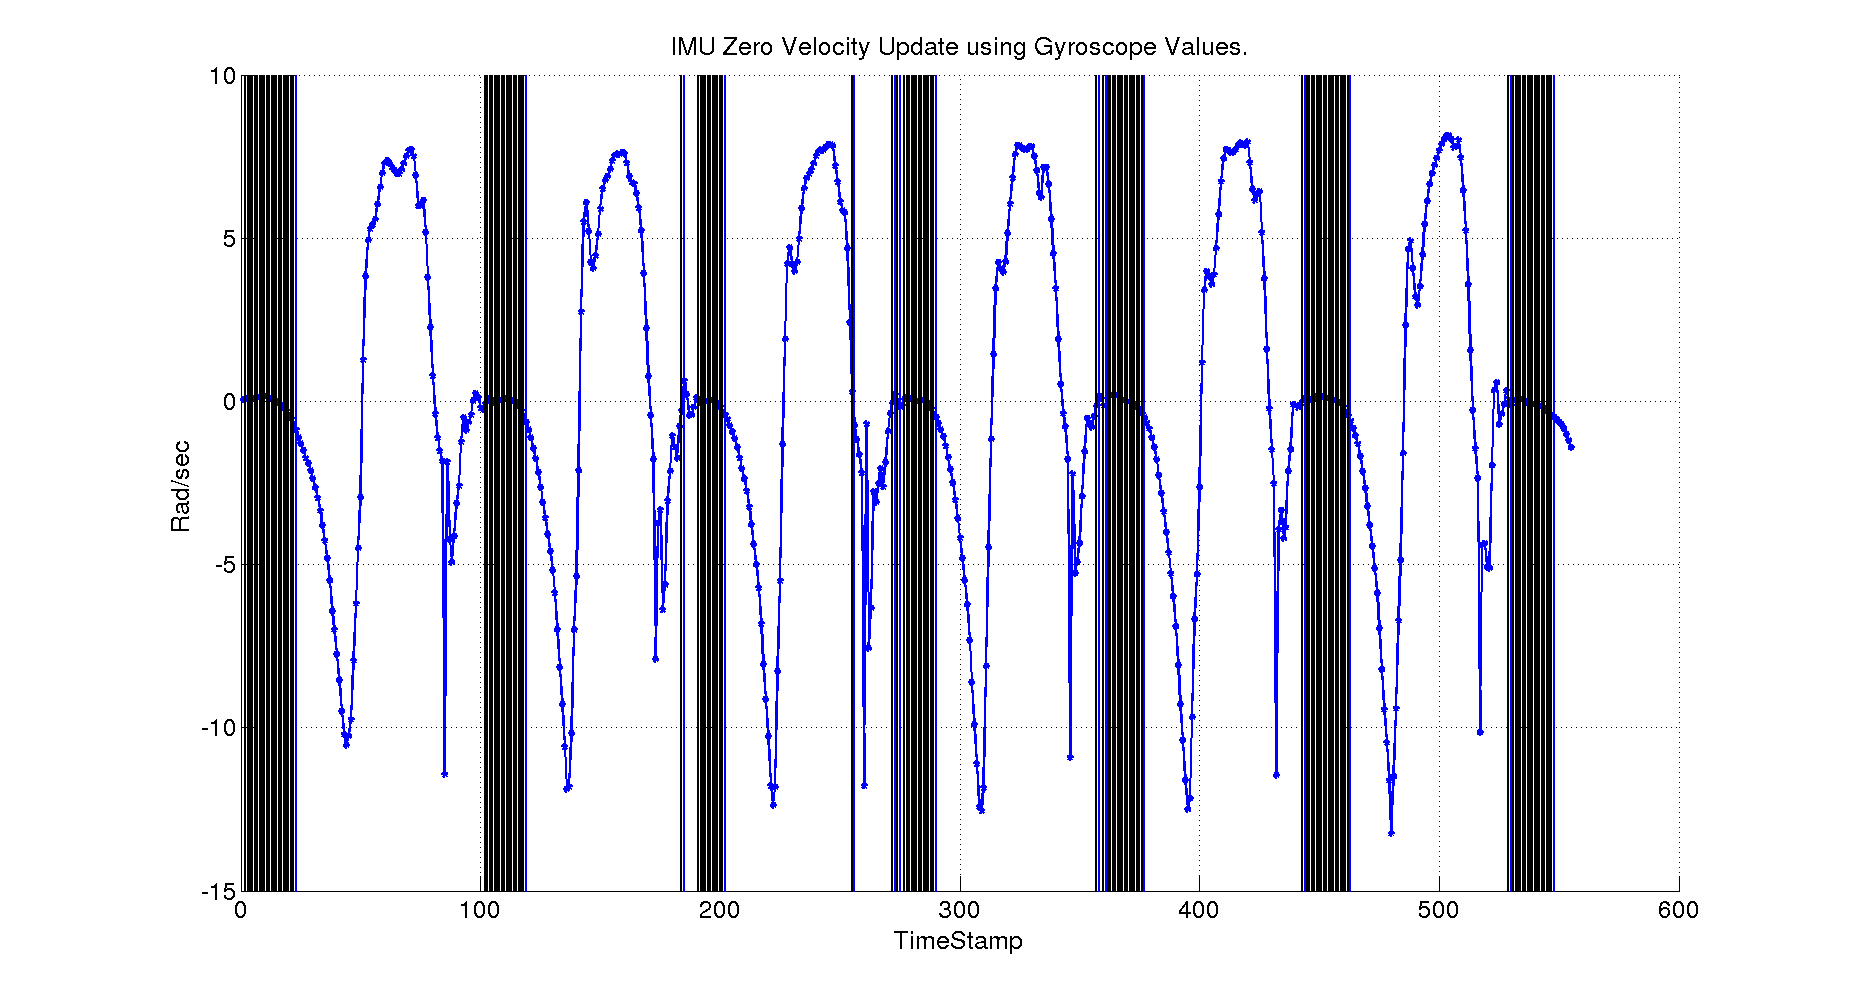
\includegraphics[scale=.3]{imuzerovelocitygyro.png}
\caption{IMU Zero Velocity Detection. Using Gyroscope Threshold}
\label{imuzerovelocitygyro}
\end{figure}

\FloatBarrier

\subsection*{Applying Update using Kalman Filter}

Before Update

\begin{figure}[!htb]
\centering
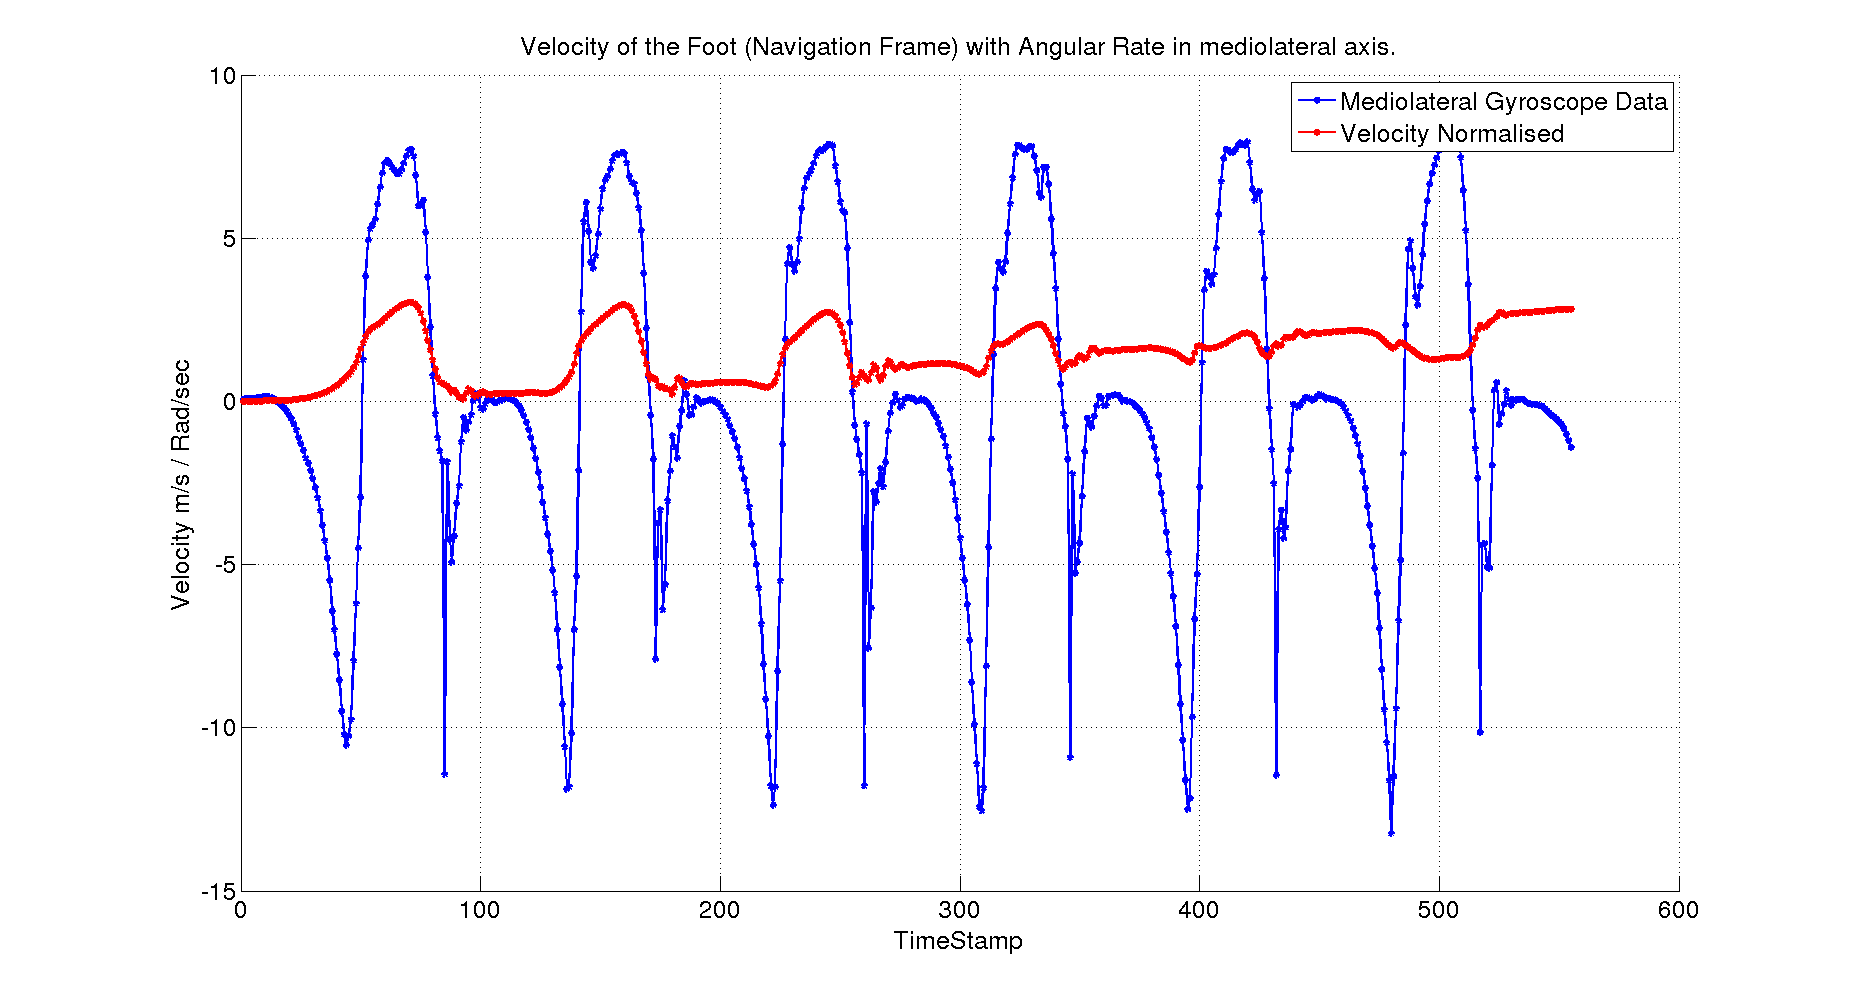
\includegraphics[scale=.3]{velocityDriftGyro.png}
\caption{Velocity with Drift and Gyroscope Data for Mediolateral Axis}
\label{velocityDriftGyro}
\end{figure}

\FloatBarrier

After Update

\begin{figure}[!htb]
\centering
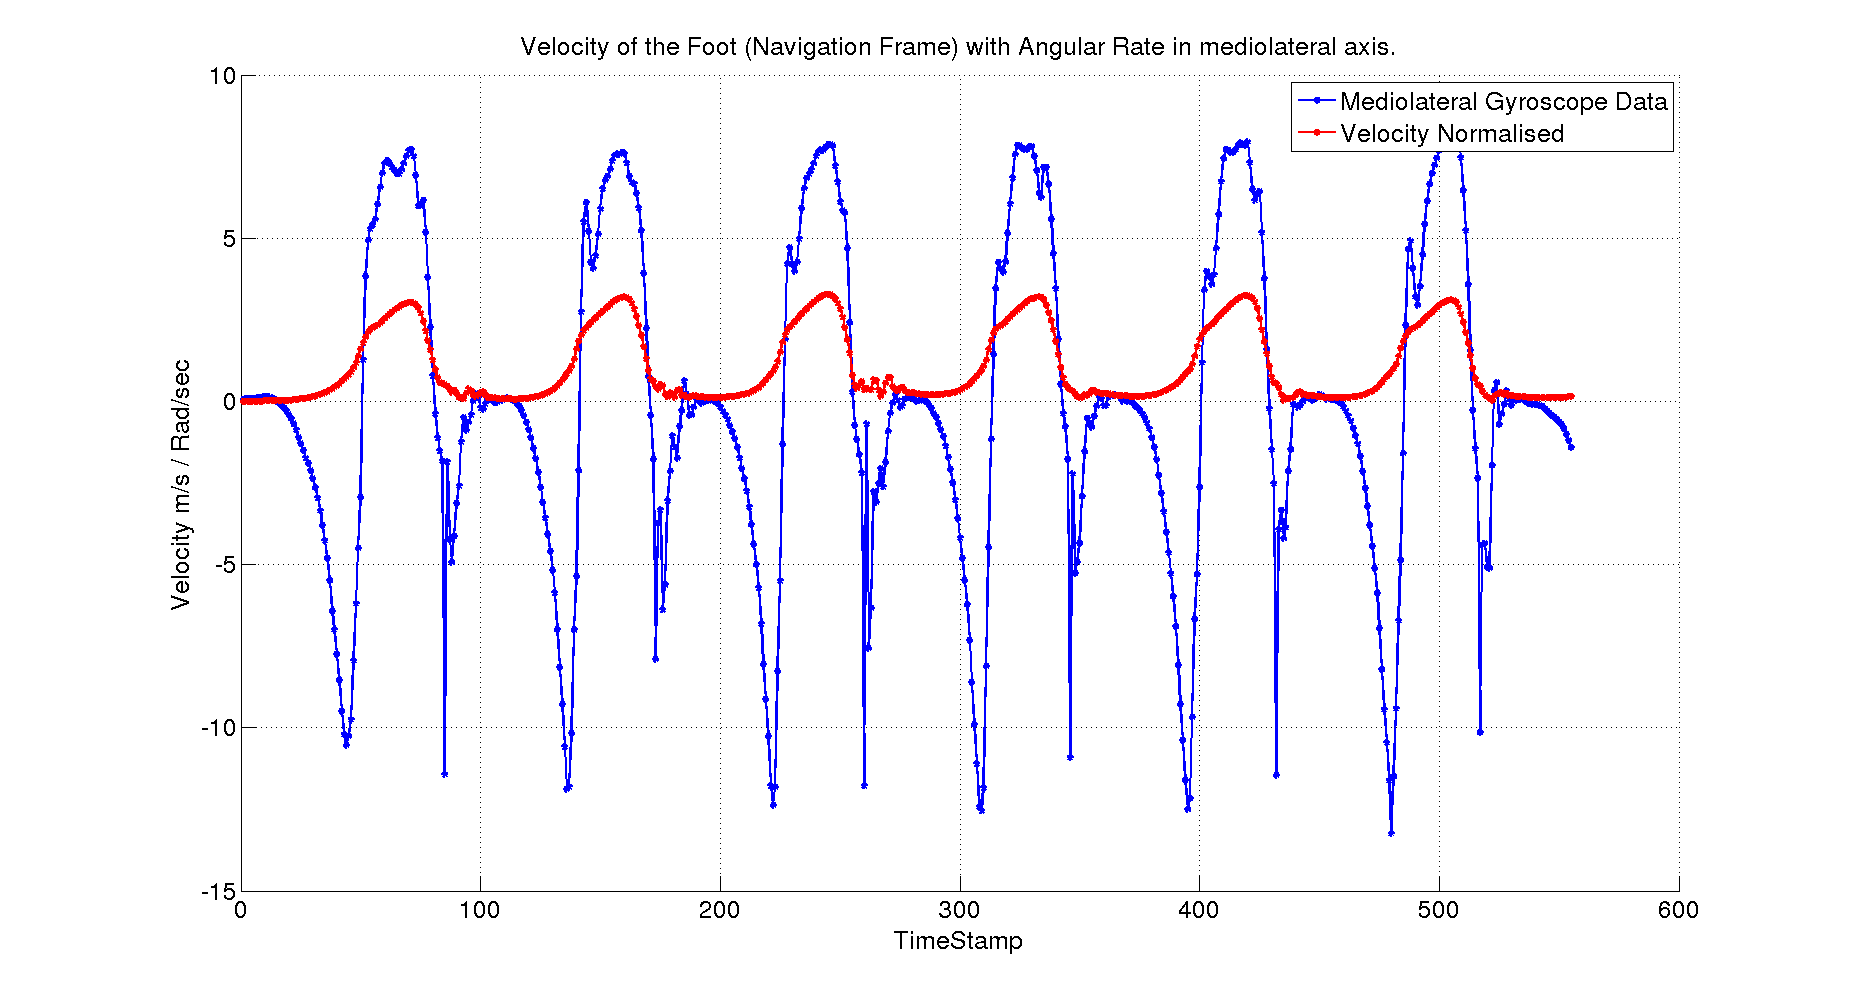
\includegraphics[scale=.3]{velocityGyro.png}
\caption{Velocity without Drift and Gyroscope Data for Mediolateral Axis}
\label{velocityGyro}
\end{figure}
\FloatBarrier

\begin{figure}[!htb]
\centering
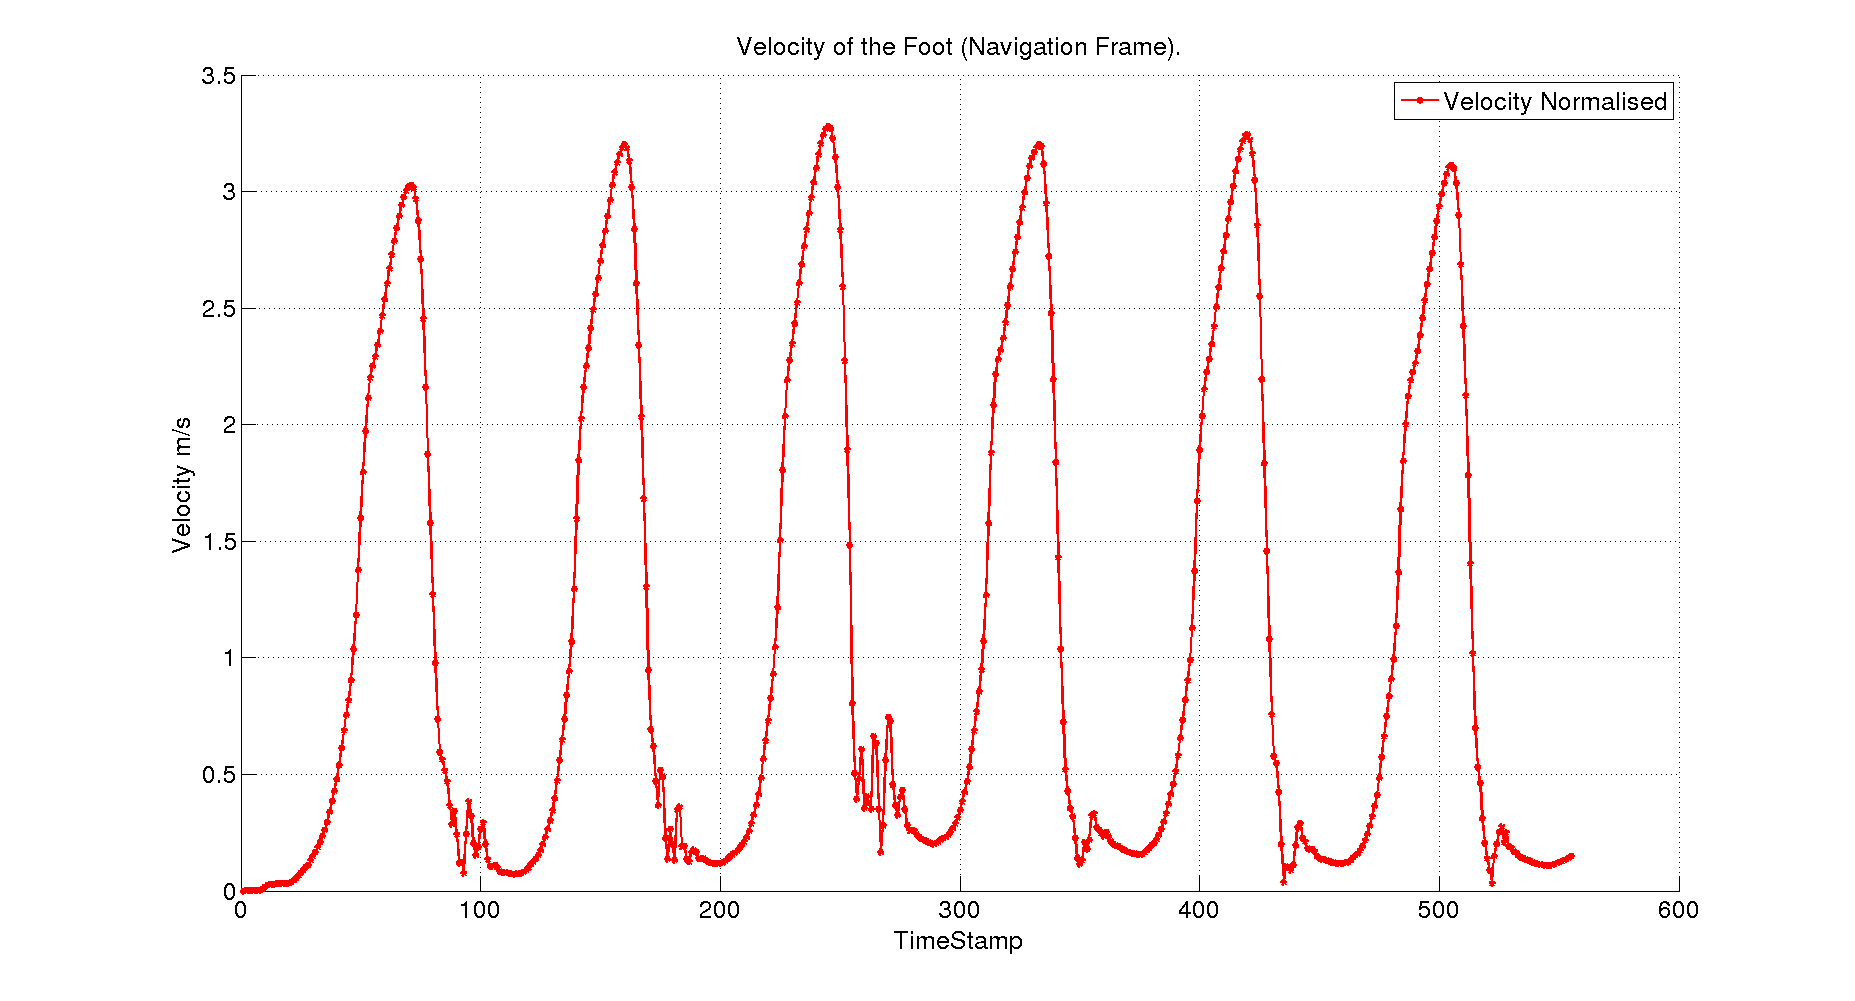
\includegraphics[scale=.3]{velocity.png}
\caption{Velocity without Drift}
\label{velocity}
\end{figure}

\FloatBarrier

Using method given in \cite{6127851}, we can calculate the path of the subject.
\begin{figure}[!htb]
\centering
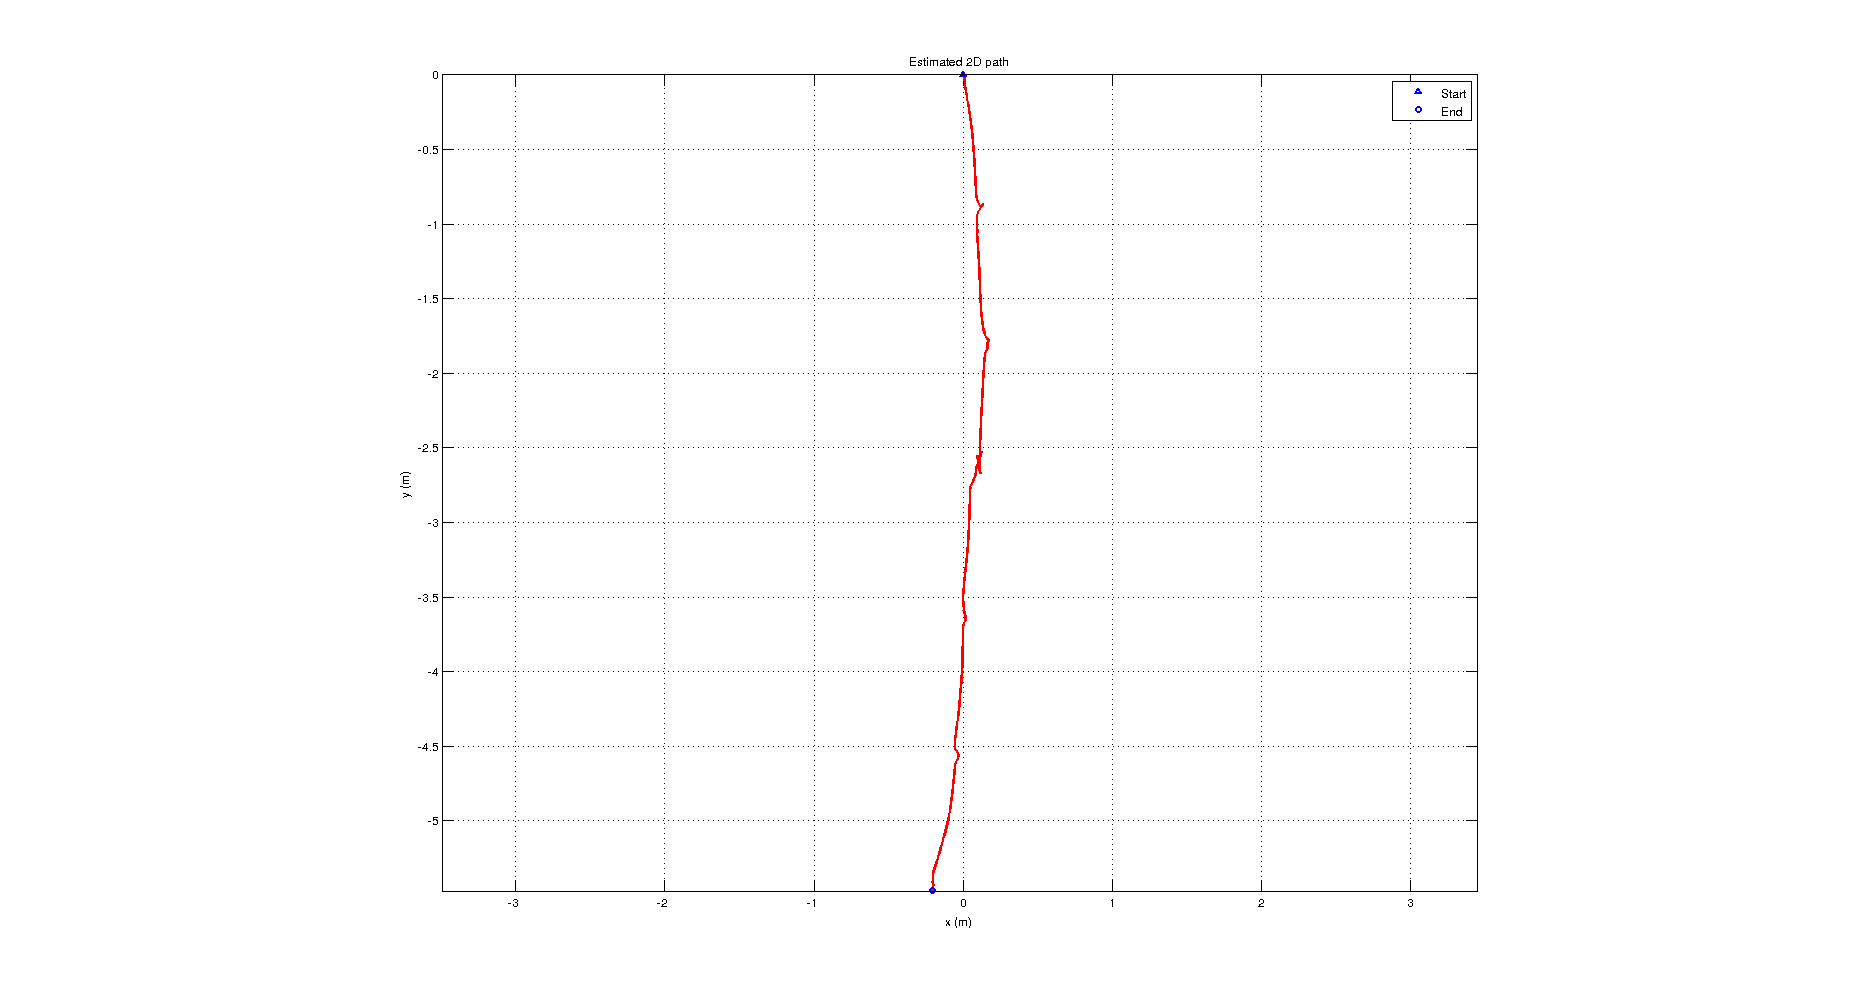
\includegraphics[scale=.35]{position.png}
\caption{Estimated 2D path}
\label{position}
\end{figure}

\FloatBarrier

\bibliography{mybib}{}
\bibliographystyle{plain}
\end{document}